We discuss the performance of the centralized algorithms in Section \ref{sec-3} for some system configurations. To begin with, we consider a single cell \ac{SISO} model operating at \me{10} dB \ac{SNR} with \me{K = 3} users sharing \me{N = 3} sub-channel resources. The number of packets waiting at the transmitter for each user is given by \me{Q_k = 4,8} and \me{4} bits, respectively. 
\begin{table*}
	\centering
		\caption{Sub-channel-wise listing of channel gains and rate allocations by different algorithms for a scheduling instant}
	\renewcommand{\arraystretch}{1.25} \scriptsize
	\begin{tabular}{|*{14}{c|}}
		\hline
		\multirow{2}{*}{Users} & \multirow{2}{*}{Queued} & \multicolumn{3}{c|}{\multirow{2}{*}{Channel Gains}} & \multicolumn{3}{c|}{Q-WSRME approach} & \multicolumn{3}{c|}{\multirow{2}{*}{JSFRA Scheme}} & \multicolumn{3}{c|}{Q-WSRM band} \\
		\multirow{2}{*}{} & \multirow{2}{*}{Packets} & \multicolumn{3}{c|}{} & \multicolumn{3}{c|}{(modified \review{\emph{backpressure}})} & \multicolumn{3}{c|}{} & \multicolumn{3}{c|}{Alloc Scheme} \\
		\cline{3-14}
		&& SC-\me{1} & SC-\me{2} & SC-\me{3} & SC-\me{1} & SC-\me{2} & SC-\me{3} & SC-\me{1} & SC-\me{2} & SC-\me{3} & SC-\me{1} & SC-\me{2} & SC-\me{3} \\
		\hline
		\me{1} & \me{4} & \me{1.71} &  \me{0.53}  &  \me{0.56} & \me{0} &  \me{0}  &  \me{0} & \me{4.0} &  \me{0}  &  \me{0} & \me{0} &  \me{0}  &  \me{0} \\
		\me{2} & \me{8} & \me{0.39} &  \me{1.41}  &  \me{1.03} & \me{0} &  \me{4.88}  &  \me{3.11} & \me{0} &  \me{5.49}  &  \me{0} & \me{0} &  \me{4.39}  &  \me{3.53} \\
		\me{3} & \me{4} & \me{2.34} &  \me{1.26}  &  \me{2.32} & \me{4.0} &  \me{0}  &  \me{0} & \me{0} &  \me{0}  &  \me{4.0} & \me{5.81} &  \me{0}  &  \me{0} \\
		\hline
		\multicolumn{5}{|c|}{Remaining backlogged packets (\me{\chi})} & \multicolumn{3}{c|}{\me{3.92} bits} & \multicolumn{3}{c|}{\me{2.51} bits} & \multicolumn{3}{c|}{\me{5.89} bits} \\
		\hline
	\end{tabular}
	\label{tbl-1} \vspace{-0.1in}
\end{table*}
\begin{figure*}
	\centering
	\subfloat[][System Model \me{\lbrace N,N_B,K,N_T,N_R \rbrace = \lbrace 4,3,9,4,1\rbrace}]{
		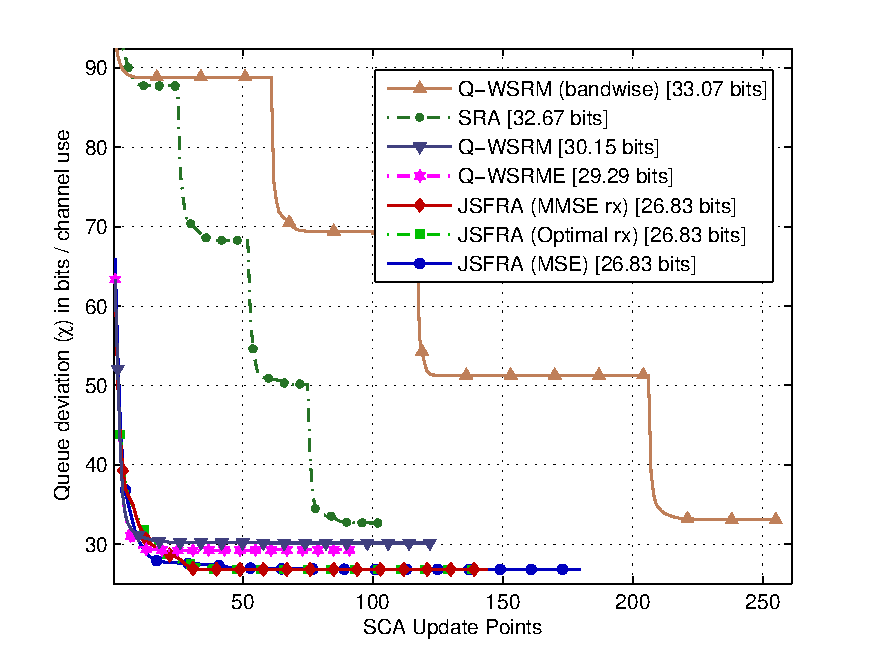
\includegraphics[width=0.5\textwidth]{fig-1-4}
		\label{fig-1}}
	\subfloat[][System Model \me{\lbrace N,N_B,K,N_T,N_R \rbrace = \lbrace 2,3,9,4,2\rbrace}]{
		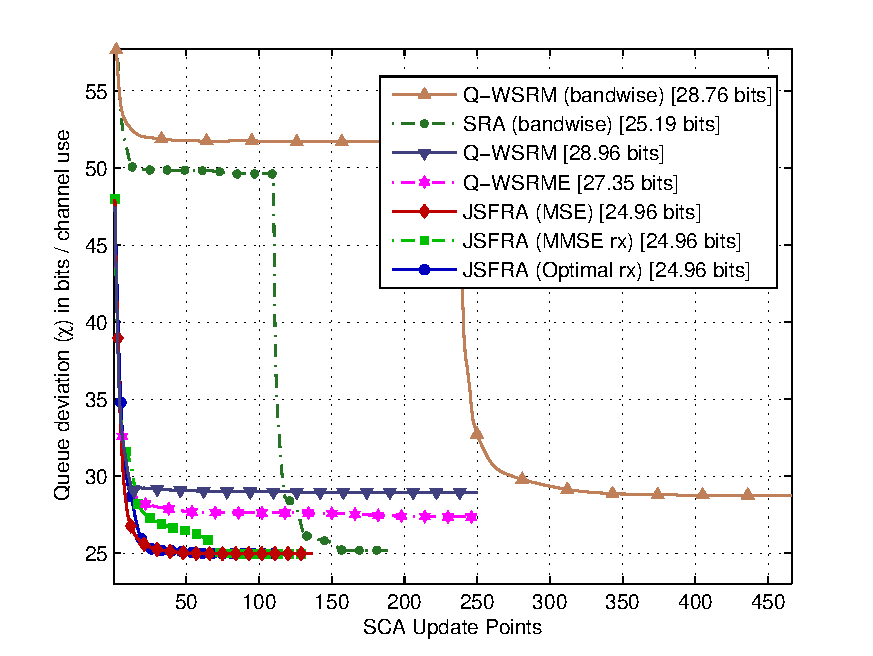
\includegraphics[width=0.5\textwidth]{fig-2-5}
		\label{fig-2}}
	\caption{Total number of backlogged packets \me{\chi} present in the system after each \ac{SCA} updates}
	\label{fig-a} \vspace{-0.1in}
\end{figure*}

Table \ref{tbl-1} tabulates the channel seen by the users over each sub-channel followed by the rates assigned by three different algorithms, \ac{Q-WSRME} allocation, \ac{JSFRA} approach and the band-wise \ac{Q-WSRM} scheme using the \ac{WMMSE} design \cite{wmmse_shi}. The performance metric used for the comparison is the total number of backlogged bits left over at each slot after the allocation, which is denoted as \me{\chi = \sum_{k = 1}^K \; [ Q_k - t_k ]^+}. Even though \me{\mc{U}(1)} and \me{\mc{U}(3)} has equal number of backlogged packets of \me{Q_{1} = Q_{3} = 4} bits, user \me{\mc{U}(3)} is scheduled in the first sub-channel due to the better channel condition. In contrast, the \ac{JSFRA} approach assigns the first user on the first sub-channel, which reduces the total number of backlogged packets waiting at the transmitter. The rate allocated for \me{\mc{U}(2)} on the second sub-channel is higher in \ac{JSFRA} scheme compared to the other schemes. It is due to the efficient allocation of the total power shared across the sub-channels.
\begin{table}
	\centering
	\caption{Number of backlogged bits associated with each user for a system \me{\lbrace N,N_B,K,N_R \rbrace = \lbrace 5,2,8,1 \rbrace}.}
	\renewcommand{\arraystretch}{1.25} \scriptsize
	\begin{tabular}{|c|*{8}{c}|c|}
		\hline
		\multirow{2}{*}{\me{q}} & \multicolumn{8}{c|}{user indices} & \multirow{2}{*}{\me{\chi}} \\
		\cline{2-9}
		& 1 & 2 & 3 & 4 & 5 & 6 & 7 & 8 & \\
		\hline
		\hline
		\me{1} & 15.0 & 3.95 & 5.26 & 8.95 & 7.0 & 11.9 & 12.0 & 9.7 & 25.15 \\
		\me{2} & 11.2 & 3.9 & 10.76 & 10.65 & 10.27 & 9.68 & 8.77 & 5.9 & 27.77 \\
		\me{\infty} & 11.4 & 4.4 & 10.4 & 10.4 & 10.4 & 8.4 &  8.4 &  6.4 & 28.68 \\
		\hline
		\me{Q_k}  & 15.0 &  8.0 &  14.0 & 14.0 &  14.0 & 12.0 & 12.0 & 10.0  \\
		\cline{1-9}
	\end{tabular}
	\label{tbl-3} \vspace{-0.1in}
\end{table}

For a \ac{MIMO} framework, we consider a system with \me{N=3} sub-channels and \me{N_B = 3} \acp{BS}, each equipped with \me{N_T = 4} transmit antennas operating at \me{10}dB \ac{SNR}, serving \me{|\mc{U}_b| = 3} users each. The path loss between the \acp{BS} and the users are uniformly generated from \me{[0,-3]} dB and the association is made by selecting the \ac{BS} with the lowest path loss component. Fig. \subref*{fig-1} shows the performance of the centralized schemes for a single receive antenna system. The total number of queued packets for Fig. \subref*{fig-1} is given by \me{Q_k = [14,15,14,8,12,9,12,11,11]} bits and for Fig. \subref*{fig-2} is \me{Q_k = [9,12,8,12,5,4,10,8,5]} bits respectively.

The performance of the centralized algorithms are compared in terms of the total number of residual bits remaining in the system after each \ac{SCA} update in Fig. \ref{fig-a}. The \ac{Q-WSRM} algorithm is not optimal due to the problem of over-allocation when the number of queued packets are few in number. In contrast, the \ac{Q-WSRME} algorithm provides more favorable allocation by including the explicit rate constraint to avoid the over-allocation. It can be seen that the \ac{JSFRA} algorithms converge to the optimal point for all formulations proposed in Section \ref{sec-3.2.1}. 

For both scenarios in Fig. \ref{fig-a}, the \ac{Q-WSRME} performs marginally inferior to the \ac{JSFRA} algorithms due to the weights used in the algorithm. The performance loss is  attributed to the fact that the \ac{Q-WSRME} algorithm favors the users with the large number of backlogged packets as compared to the users with better channel conditions. Fig. \subref*{fig-2} compares the algorithms for \me{N_R = 2} receive antenna case. In all figures, the receivers are updated along with the \ac{SCA} update instants \textit{i.e}, \me{J_{\max} = 1} in Algorithm \ref{algo-1}. It is also noted that the performance degradation by performing the group update is very minimal. Since the receiver minimizes the objective for the fixed transmit precoders, the convergence is monotonic as can be seen from the figures.

The behavior of the \ac{JSFRA} algorithm for different exponents \me{q} is outlined in the Table \ref{tbl-3} for the users located at the cell-edge of the system employing \me{N_T = 4} transmit antennas. It is evident that the \ac{JSFRA} algorithm minimizes the total number of queued bits for the \me{\ell_1} norm compared to the \me{\ell_2} norm, which is shown in the column displaying the total number of left over packets \me{\chi} in bits. The \me{\ell_{\infty}} norm provides fair allocation of the resources by making the left over packets to be equal for all users to \me{\chi_k = 3.58} bits.
